\documentclass[a4paper, 12pt]{ctexart}

%%%%%% 导入包 %%%%%%
\usepackage{graphicx}         %插入图片要用到的宏包
\usepackage{geometry}         %设置页边距要用到的宏包
\usepackage{xcolor}           %设置颜色相关的宏包
\usepackage{cite}
\usepackage{amsmath}          %和下面一个宏包一样 都是输入数学公式要用到的宏包
\usepackage{amssymb}
\usepackage[colorlinks=red]{hyperref}
\usepackage{bbding}           %这个宏包可以输入一些特殊字符 给文档增色
\usepackage{multirow}         %表格排版要用到的宏包

%%%%%% 设置页边距 %%%%%%
\geometry{left=2.2cm,right=2.2cm,top=2.54cm,bottom=2.54cm}

%%%%%% 设置字号 %%%%%%
\newcommand{\chuhao}{\fontsize{42pt}{\baselineskip}\selectfont}
\newcommand{\xiaochuhao}{\fontsize{36pt}{\baselineskip}\selectfont}
\newcommand{\yihao}{\fontsize{28pt}{\baselineskip}\selectfont}
\newcommand{\erhao}{\fontsize{21pt}{\baselineskip}\selectfont}
\newcommand{\xiaoerhao}{\fontsize{18pt}{\baselineskip}\selectfont}
\newcommand{\sanhao}{\fontsize{15.75pt}{\baselineskip}\selectfont}
\newcommand{\sihao}{\fontsize{14pt}{\baselineskip}\selectfont}
\newcommand{\xiaosihao}{\fontsize{12pt}{\baselineskip}\selectfont}
\newcommand{\wuhao}{\fontsize{10.5pt}{\baselineskip}\selectfont}
\newcommand{\xiaowuhao}{\fontsize{9pt}{\baselineskip}\selectfont}
\newcommand{\liuhao}{\fontsize{7.875pt}{\baselineskip}\selectfont}
\newcommand{\qihao}{\fontsize{5.25pt}{\baselineskip}\selectfont}


%%%% 定理类环境的定义 %%%%
\newtheorem{example}{例}             % 整体编号
\newtheorem{algorithm}{算法}
\newtheorem{theorem}{定理}[section]  % 按 section 编号
\newtheorem{definition}{定义}
\newtheorem{axiom}{公理}
\newtheorem{property}{性质}
\newtheorem{proposition}{命题}
\newtheorem{lemma}{引理}
\newtheorem{corollary}{推论}
\newtheorem{remark}{注解}
\newtheorem{condition}{条件}
\newtheorem{conclusion}{结论}
\newtheorem{assumption}{假设}

%%%% 重定义 %%%%
\renewcommand{\contentsname}{目录}  % 将Contents改为目录
\renewcommand{\abstractname}{摘要}  % 将Abstract改为摘要
\renewcommand{\refname}{参考文献}   % 将References改为参考文献
\renewcommand{\indexname}{索引}
\renewcommand{\figurename}{图}
\renewcommand{\tablename}{表}
\renewcommand{\appendixname}{附录}
\renewcommand{\algorithm}{算法}

%%%% 下面的命令让页码居中 %%%%
\pagestyle{plain}

%%%% 下面的命令设置行间距与段落间距 %%%%
\linespread{1.4}
\setlength{\parskip}{0.5\baselineskip}


%%%% 定义标题格式,包括title,author,affiliation,email等 %%%%
\title{投资指标参数}
\author{张三\footnote{电子邮件: zhangsan@gmail.com}\\[2ex]
\xiaosihao 中山大学数据科学与计算机学院\\[2ex]
}
\date{2015年11月25日}

%以上都是一些预设命令 只改变文档的输出效果 不产生实际输出
%**************************************************

%%%% 正文开始 %%%%
\begin{document}
\maketitle             %生成标题页
%%%% 以下这两行的命令的效果是让标题页不出现页码 %%%%
%--------------------------------------------------
\setcounter{page}{0}
\thispagestyle{empty}
%--------------------------------------------------

\newpage               %另起一页输入正文

%----------------------------------------------------------------------------------------------------
%%%% 由于这是一份简短的报告 所以 '节' '小结' 等文档结构我就没有
%%%% 用\section \subsection 等命令来生成 用这些命令生成的标题会
%%%% 有编号 在中文排版中不好改 所以我用以下命令来自己生成标题
%%%% \hspace{}  ---> 设置水平间距 'em'代表一个大写字母 'M' 的宽带 
%%%% \textbf{}  ---> 加粗字体
%%%% \xiaosihao ---> 设置字体大小 各种字号在前面已经定义好 
\hspace{-2em}\textbf{\sihao 一、第一节标题}

在这里输入你的内容。这这是测试文本,这是测试文本,这是测试文本,这是测试文本,这是测试文本,这是测试文本,是测试文本。

如果要另起一段,在源码中要空一行。如果空了多行,LaTex也只会考虑一行而忽略其他行。要另起一段就空一行吧。

\vspace{-3ex}     %这个命令是设置垂直间距 'ex'代表一个大写字母 'X' 的高度
%%%% 这是一个列表环境 生成列表 
%%%% \itemindent ---> 设置每一项的缩进量
%%%% \itemsep    ---> 设置列表项间的间距
\begin{itemize}\setlength{\itemindent}{1em}\setlength{\itemsep}{0.3ex}
    \item LaTex is good.
    \item LaTex is not bad.
    \item LaTex is good and not bad.
\end{itemize}
%----------------------------------------------------------------------------------------------------

%----------------------------------------------------------------------------------------------------
\vspace{2ex}
\hspace{-2em}\textbf{\sihao 二、第二节标题}

%%%% 用bbding这个宏包可以输入一些特殊字符 
%%%% \HandRight ---> 输入一个指向右边的手性 可以用来标记标题
%%%% \,         ---> 产生一个空格 可用\hspace{}来达到相同的效果
\hspace{-2em}\HandRight\, \textbf{子标题1}

子标题1下的内容。

\hspace{-2em}\HandRight\, \textbf{子标题2}

子标题2下的内容。

\vspace{3ex}
%%%% \includegraphics ---> 用来插入图片 png jpeg等均可
%%%% scale            ---> 参数 对图片进行缩放
%%%% fc.png           ---> 图片文件名 如果和源文件不在同一目录下 给出绝对路径
%%%% \centerline{}    ---> 让图片居中 让文本居中也常用此命令
\centerline{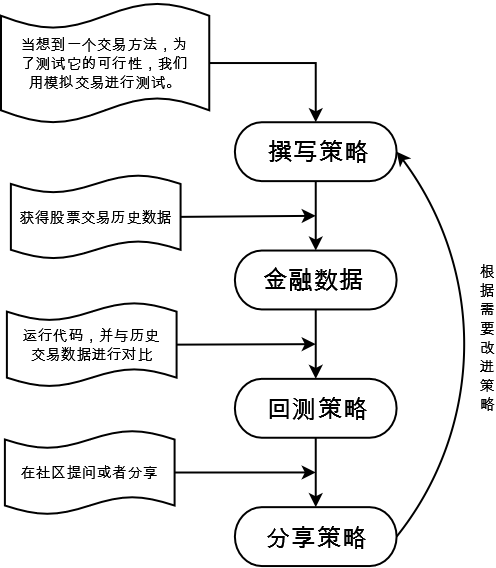
\includegraphics[scale=0.2]{fc.png}}  

\hspace{-2em}\HandRight\, \textbf{子标题3}

\newcommand{\tabincell}[2]{\begin{tabular}{@{}#1@{}}#2\end{tabular}}  %这是让表格内容可以换行 
%%%% 生成表格的环境
%%%%
\begin{table}[h!]    %这是浮动体环境
    \center          %让表格居中哦
    \small           %设置表格的字号
    \begin{tabular}{|c|c|c|c|c|c|}    %表格有多少列在这里指定 'c'表示内容居中 同理有参数 'l' 和 'r'
        \hline       %产生水平横线
        LaTex & LaTex & LaTex                                & LaTex                                & LaTex & LaTex \\
        \hline
        LaTex & LaTex & \tabincell{c}{内容比较多\\ 我要换行} & \tabincell{c}{内容比较多\\ 我要换行} & LaTex & LaTex \\
        \hline
    \end{tabular}
\end{table}
%----------------------------------------------------------------------------------------------------

\textbf{三、第三节}

\end{document}

